
\chapter{Bibliothèque Scheme}
%% Bonne place???
Le langage Scheme supporte plusieurs paradigme de programmation comme
la programmation fonctionnel et impérative. La syntaxe de ce langage
est basé sur les s-expressions, qui consiste en des listes parenthésés.
Un programme Scheme est donc une séquence de listes. Les listes sont
aussi une structure principale du langage. Le langage Scheme peut facilement
manipuler dynamiquement du code puisque le code utilise principalement des listes.

\subsection{Fonction et Procédure}
Les procédures en Scheme sont définit par la forme spécial \lstcode{(lambda args body)}.
Les éléments \lstcode{args} et \lstcode{body} correspondent respectivement à la liste
d'arguments et au corps de la procédure. Pour définir une procédure globalement il faut
ajouter une définition avec la forme \lstcode{(define sym val)} qui permet d'associer le
symbole \lstcode{sym} à la valeur \lstcode{val}.

\begin{figure}[ht]
  \begin{center}
    \begin{mplisting}{0.25}
(define abs
  (lambda (x)
    (if (< x 0)
      (- x)
      x)))
\end{mplisting}
  \end{center}
  \caption{Exemple d'utilisation des forme spécial \lstcode{define} et \lstcode{lambda} dans
  la définition d'une fonction qui retourne le résultat de la valeur absolue d'un nombre.}
\end{figure}

% READ Distinguer macro procedure.
En Scheme les procédure sont des objet de première classe, cela signifie qu'il
peuvent être passé en argument ou retourné d'une fonction. Ils manipulent des
valeurs.  Les procédure et les fonction définit par la forme spéciale
\lstcode{define} sont accessible à la phase d'exécution.

\subsection{Macro}
Le langage Scheme offre des constructions qui permettent la transformation
du code source. Ce sont les macros, certain langage comme C et C++ offre un système
de préprocesseur qui ce limite à une simple substitution textuelle. Les macros en Scheme
sont des procédure Scheme avec toute les capacités de calcule.

Les macros sont une forme de procédure qui manipule la structure du code
plutôt que des valeurs. Il sont définit soit par la forme \lstcode{define-macro}
où \lstcode{define-syntax}.

%% XXX: suite.

La structure des bibliothèque définit dans le depuis le standard
R4RS\cite{Scheme:R4RS} et R5RS\cite{Scheme:R5RS} consistait simplement de
fichiers Scheme qui sont importés dans le module courant. Cette importation est
effectué soit par la procédure \texttt{load} ou par la forme spéciale
\texttt{include}. Ce modèle de bibliothèque possède plusieurs lacunes.

%% Gambit doc
\begin{itemize}
  \item Ce modèle de chargement n'est pas à l'abri des chargements multiples
    d'un module qui amène soit la duplication de code ou la réévaluation
    non désiré d'un code.

  \item Toutes les déclarations dans un module sont ajoutés à l'environnement
    global lors de l'importation. Cela amène des conflits de nom entre les
    symboles du module principale et les modules importés.

  \item L'importation d'un module par \texttt{load} nécessite le chemin exacte
    du module à importer qui peut être soit relatif ou absolu.  Un chemin
    relatif prend comme origine le répertoire présent.  L'importation d'un
    module par \texttt{include}, contrairement au \texttt{load}, le chemin
    relatif prend comme origine l'emplacement du fichier dans lequel la forme
    spécial \texttt{include} ce situe.

\end{itemize}


Lors d'un chargement de bibliothèque par \texttt{load} les macros sont expansé
et le code résultant est exécuté. Pour avoir accès aux macros, il faut utiliser la
forme spécial \texttt{include} qui est expansé par le contenu du fichier.
L'expression \lstcode{(include "foo#.scm")} est remplacé par le contenu du fichier
\lstcode{foo#.scm}. L'inclusion tout comme un \lstcode{load} nécessite le chemin
absolu ou relatif du fichier. L'exemple \ref{fig:r4rs_fact} montre un exemple
de module simple n'utilisant que \lstcode{load}.

\begin{figure}[ht]
  \begin{center}
    \begin{tabular}{|l|}
    \hline
    \begin{mplisting}{0.4}
;; fact.scm
(define (fact n)
  (if (< n 2)
    n
    (* n (fact (- n 1)))))
\end{mplisting} \\\hline
    \begin{mplisting}{0.4}
;; main.scm
(load "fact.scm")
(display (fact 5))
\end{mplisting} \\\hline
    \end{tabular}
  \end{center}
  \caption{Le fichier \texttt{fact.scm} est un exemple de module R4RS exposant
  la fonction mathématique \lstcode{fact}. Le fichier \texttt{main.scm} est un
  programme principal qui utilise le module \texttt{fact.scm}.}
  \label{fig:r4rs_fact}
\end{figure}

Le modèle de bibliothèque utilisé dans les standard Scheme prior au
R6RS\cite{Scheme:R6RS} a comme désavantage qu'une bibliothèque peut masquer les
fonctionnalités d'une autre bibliothèque puisque le chargement effectué par la
procédure \texttt{load} est dans le contexte global. Bref, les procédures de la
bibliothèque \textbf{A} peuvent rentrer en conflit de nom avec les procédures
de la bibliothèque \textbf{B} s'ils sont chargé dans le même contexte.  Pour
évité ces conflit, il faut que chaque nom utilisé au sein des bibliothèques
soit distinct, ce qui rajoute une tâche au programmeur.

\todo{Citation to gambit}

Gambit offre un mécanisme pour aider a minimiser les conflits de nom. Ce
méchanisme permet d'associer un identifiant à un autre avec la forme spécial
\lstcode{##namespace}.  L'appel à \lstcode{(##namespace ("foo#" A B))} indique
qu'une référence succécante à \lstcode{A} devient une référence à
\lstcode{foo#A} et l'un à \lstcode{B} devient une à \lstcode{foo#B}. Le espace
de nom dans lequel \lstcode{A} et \lstcode{B} est \lstcode{foo#}.

\begin{center}
  \begin{figure}[h]
  \begin{tabular}{|l|}
\hline
\begin{mplisting}{0.5}
;; math#.scm
(##namespace ("math#" fact fib))
\end{mplisting} \\\hline
\begin{mplisting}{0.6}
;; math.scm
(##namespace ("math#" fact fib))
(define (fib n)
  (if (< n 2)
    n
    (+ (fib (- n 1)) (fib (- n 2)))))
(define (fact n)
  (if (< n 2)
    1
    (* n (fact (- n 1)))))
\end{mplisting}\\\hline
  \end{tabular}
  \caption{Écriture d'un petit module mathématique qui implémente les fonctions \lstcode{fact}
    et \lstcode{fib}. Ce module est séparé en 2 fichiers, \texttt{math\#.scm} est un fichier
    contenant les déclarations de l'espace de noms et des définitions de macros que le module
    exporte.}
  \label{fig:math_module1}
\end{figure}
\end{center}


Le concept de bibliothèque a été raffiné  dans le R6RS.  Le R6RS rend le
support de la procédure \texttt{load} optionnel et ajoute une forme spéciale
\texttt{library} pour définir des bibliothèques et une autre forme spéciale
\texttt{import} pour gérer la inclure une bibliothèque.  Les noms utilise
pour nommer une bibliothèque peuvent seulement contenir des symboles et des
numéros de versions à la fin. Les expression import et export doivent seulement
apparaître une seul fois dans le définition de la bibliothèques.

Les bibliothèques ainsi définit, lie chaque procédure à la bibliothèque.  Cela
permet la réutilisation des mêmes identificateurs dans deux bibliothèque
différente.  Les conflits de nom sont gérés lors de l'importation des la
bibliothèques. L'importation d'un module est permit au sein d'une bibliothèque
comme dans un programme principale. La syntaxe d'un import reste identique dans
ces deux cas.


%\begin{center}
%  \begin{figure}[h]
%  \begin{tabular}{|l|l|}
%\hline
%\begin{mplisting}{0.5}
%;; Library
%(library (math)
%  (export fact)
%  (import (rnrs base))
%  (define (fact n)
%    (if (< n 2)
%      1
%      (* n (fact (- n 1))))))
%\end{mplisting} &
%\begin{mplisting}{0.5}
%;; Main program
%(import
%  (rnrs base)
%  (rnrs io simple)
%  (math))
%
%(display (fact 5))
%(newline)
%\end{mplisting}\\\hline
%  \end{tabular}
%\caption{À gauche, il y a un exemple d'une bibliothèque mathématique dans le format R6RS qui implémente
%la fonction factoriel. À droite, un exemple d'importation de la bibliothèques qui utilise la forme
%spéciale \texttt{import}.}
%\end{figure}
%\end{center}

L'implémentation des bibliothèques Scheme est basé sur le standard R7RS qui
conserve la procédure \texttt{load} que le R6RS enlève et remplace la structure
des bibliothèques.  Une bibliothèque en R7RS utilise la forme spécial
\texttt{define-library} au lieu de \texttt{library}. Ces deux formes ont
beaucoup de similarité, il n'est pas difficile de passé d'une bibliothèque R6RS
à une bibliothèque R7RS. Takashi Kato a publié un article au \emph{Scheme
Workshop} 2014 qui explique une procédure pour transformer un module R6RS en
R7RS \cite{SW2014:R6RS/to/R7RS}.  L'extension de fichier utilisé par les
définitions des bibliothèques est \verb|.sld| qui signifie \emph{Scheme Library
Definition}.

\begin{center}
  \begin{figure}[h]
  \begin{tabular}{|l|l|}
    \hline
    \begin{mplisting}{0.5}
;; Library R6RS
(library (math)
  (export fact)
  (import (rnrs base))
  (define (fact n)
    (if (< n 2)
      1
      (* n (fact (- n 1))))))
\end{mplisting} &
    \begin{mplisting}{0.5}
;; Library R7RS
(define-library (math)
  (export fact)
  (import (scheme base))
  (begin
    (define (fact n)
      (if (< n 2)
        1
        (* n (fact (- n 1)))))))
\end{mplisting}\\\hline
  \end{tabular}
\caption{À gauche, il y a un exemple d'une bibliothèque mathématique dans le format R6RS qui implémente
la fonction factoriel. À droite, une réécriture de la bibliothèque de gauche en R7RS.}
  \label{fig:r6rs_r7rs_math_mdoule}
\end{figure}
\end{center}

La syntaxe \lstinline{import} définit dans le R7RS indique le nom de
de la bibliothèque à collecter en plus des information sur les composante
à importer.
\begin{figure}[ht]
  \begin{mplisting}{0.9}
(import (only (gambit thread) make-thread thread-start! thread-join!))
\end{mplisting}
  \caption{Importation d'un sous-ensemble des fonctionnalité de la bibliothèque}
\end{figure}

% - (import (foo)) ; exportant f1 f2 f3
% ===>
% - (##demand-module foo)
% - (##namespace ("foo") f1 f2 f3)
% - macros
% - (##namespace (""))

\section{Chargement des bibliothèques}


Un système est composé d'un ensemble d'éléments (modules) qui interagissent
entre eux.  Une bibliothèque fait office de module au sein d'un système simple
ou complexe.
%La collection des modules s'effectue au sein d'un

% TODO: voir chargé
Le chargement d'une bibliothèque Scheme (ou module) est séparé en plusieurs niveaux.
% TODO: now
Les bibliothèques sont soit lu du disque vers la mémoire durant l'exécution
ou déjà dans la mémoire du processus. Durant la compilation les modules sont
collecté pour construire un exécutable. Le chargement
d'une bibliothèque inclut une phase de recherche sur le système de fichier pour valider
l'existence de la bibliothèque et des fonctionnalités demandés. L'emplacement des
bibliothèques sur le système de fichier est lié par défaut aux chemin spécifié par
le \lstinline{##module-search-order} a comme défaut \lstinline{~~lib} et \lstinline{~~userlib}.


La procédure exacte de chargement des bibliothèques par \verb|import|
n'est pas spécifier par le standard R7RS. Le standard spécifie seulement la syntaxe
à utilisé et le de comportement principal qui est
requis. L'importation d'une bibliothèque doit chargé la bibliothèque
et rendre c'est fonctionnalité disponible dans le contexte
l'importation a eu lieu qui peut soit ovenir d'un programme principale
ou d'une bibliothèque.

Le chargement d'une bibliothèque peut-être effectuée à l'exécution par
l'utilisation de \texttt{eval} (par \texttt{load}) pour les fichiers source et
\texttt{load-objcet-file} pour les bibliothèques compilées. Cette recherche
peut aussi avoir lieu durant l'édition des lien en utilisant les méta-infos
contenus dans les \textbf{.c} qui sont chacun compilé par le compilateur C
en \textbf{.o} et lié par le \textit{linker}.

\section{Modèle dynamique}
Dans ce modèle les bibliothèques sont lié au programme durant l'exécution. Cela
nécessite que les bibliothèques soit organisé sur le système de fichier d'une façon
distingable. Chaque module doit posséder un nom unique qui permet d'y référer.
Ce nom unique va être utilisé lors de la collection des dépendances.


%Les bibliothèques
%sont soit en code source ou compilé nativement avec l'extension (\textit{.oN})
%où le N correspond à la version du binaire qui commence à 1.


La recherche des bibliothèques est éffectué dans un ordre spécifique
indépendant de la spécification.  L'algorithme de recherche les bibliothèques
prend entré le nom de la bibliothèque et retourne le chemin absolu
correspondant à sont emplacement dans l'arborescence du système de fichier. Les
bibliothèques sont situées dans différents répertoires l'origine du programme,
le répertoire des bibliothèques système (\lstinline{~~lib}) et le
répertoire de bibliothèque utilisateur (\lstinline{~~userlib}).

% \begin{itemize}
%   %% XXX: directory where the executable is located (usefull for devel no need to install the module). collecté
%   \item \verb|origin/dummy.sld|
%   \item \verb|origin/dummy/dummy.sld|
%   \item \verb|~~userlib/dummy.sld|
%   \item \verb|~~userlib/dummy/dummy.sld|
%   \item \verb|~~lib/dummy.sld|
%   \item \verb|~~lib/dummy/dummy.sld|
% \end{itemize}

Chaque module possède trois niveau d'initialisation dans le système numéroté de
0 à 2. Le niveau 0 indique que le module n'a pas été initialisé. Ces les niveau
des module qui ont juste été collecté par le système. Le niveau 1 indique que
le descripteur du module à été récupéré. L'étape 2 est utilisé pour indiquer
les module chargé.

Soit un système avec les dépendance suivante:
\begin{figure}[ht]
  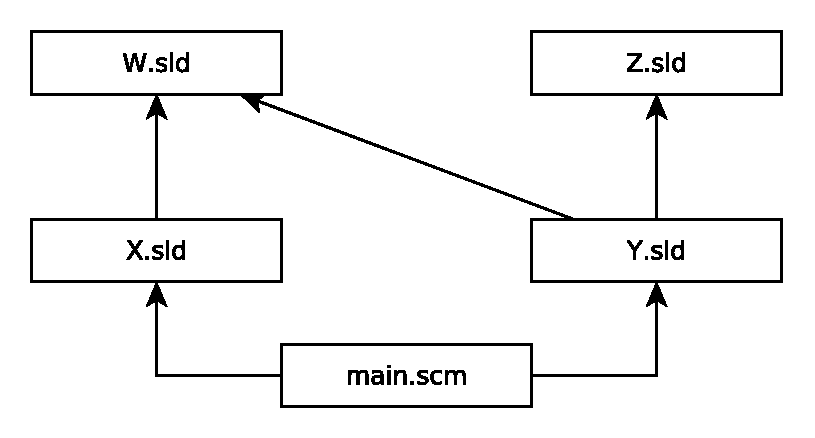
\includegraphics{figures/system-example}
  \caption{Un exemple d'un système fictif composé de différents modules.
  Le module principale se nomme utilise l'extension \textbf{.scm}
  et les bibliothèques porte l'extension \textbf{.sld}}
\end{figure} % TODO: use yed for that graph


Le démarrage du module principal Main.scm déclenche la collection des modules X
et Y, qui récursivement déclenche la collection de W et Z. L'algorithme de
collection des modules ignore les module qui apparaisse plusieurs fois au sein
du graphe.

Une fois la collection de tous ces modules est complété le descripteur de
module est récupéré par un appels à \verb|dlopen| et \verb|dlsym| dans le cas
compilé.


\section{Module hébergé}

Un module qui est hébergé est un module qui dont son contenu
se retrouve sur un domain comme \url{github.com}.


\begin{figure}[ht]
\begin{lstlisting}
hostname      = +( domainlabel "." ) toplabel
domainlabel   = alphanum | alphanum *( alphanum | "-" ) alphanum
toplabel      = alpha | alpha *( alphanum | "-" ) alphanum
alphanum      = alpha | digit
alpha         = [a-zA-Z]
digit         = [0-9]
\end{lstlisting}
  \caption{Grammaire BNF représentant un hostname selon un sous
  ensemble du RFC-2396.}
\end{figure}

La différence avec la spécification du hostname dans le RFC-2396
est que le hostname ne peut pas finir par un point et doit contenir
au moins un \verb|domainlabel|. C'est pour permettre de distingué
un module local et un module hébergé.

\subsection{Module gambit/git}

Ce module offre un interface pour utiliser interagir avec les des dépôts git.
Il permet de cloner un dépôts qui est hébergé sur \url{github.com}. Un clone du
dépôts est simplement un copie qui contient les informations suffisantes pour
passer d'une version d'un module à un autre. L'opération qui permet de changer
de version est \emph{checkout}.


%-------------------------------------------------------------------------------
%
%Modèle "link dynamique" :
%  recherche des libs au run time, utilisation de eval (par load) et
%  load-object-file
%
%  % gsi main.scm      ou      % gsc main.scm ; gsi main.o1
%
%    origin/main.scm    : (import X Y)
%          /X/X.sld     : (import)
%
% ~~userlib/Y/Y.sld     : (import Z)
%
%     ~~lib/Z/Z.sld     : (import)
%          /Z.o1
%
%-------------------------------------------------------------------------------
%
%Modèle "link statique" :
%  recherche des libs au link time en utilisant les méta-infos
%  dans les .c (demand-lib et supply-lib), chaque .c compilé en
%  un .o séparément et les .o linkés par le compilateur C
%
%  % gsc -obj -keep-c X.sld      ;; créer .c et .o
%  % gsc -obj -keep-c Y.sld      ;; créer .c et .o
%  % gsc -obj -keep-c Z.sld      ;; créer .c et .o
%  % gsc -obj -keep-c main.scm   ;; créer .c et .o
%  % gsc -exe main.c             ;; combine les .o pour créer main.exe
%
%    origin/main.scm    : (import X Y)
%          /main.c      : (demand-lib X Y)
%          /main.o
%          /X/X.sld     : (import)
%            /X.c       : (demand-lib) (supply-lib X)
%            /X.o
%
% ~~userlib/Y/Y.sld     : (import Z)
%          /Y/Y.c       : (demand-lib Z) (supply-lib Y)
%          /Y/Y.o
%
%     ~~lib/Z/Z.sld     : (import)
%          /Z/Z.c       : (demand-lib) (supply-lib Z)
%          /Z/Z.o
%
%-------------------------------------------------------------------------------
%
%Modèle "whole-program" :
%  recherche des libs au compile time en utilisant les imports
%  dans les fichiers sources, les AST de toutes les libs fusionnées
%  en un seul AST compilé par gsc (donc un seul .c généré et compilé
%  par le compilateur C pour créer main.exe)
%
%  % gsc -exe -whole-program main.scm
%
%    origin/main.scm    : (import X Y)
%          /X/X.sld     : (import)
%
% ~~userlib/Y/Y.sld     : (import Z)
%
%     ~~lib/Z/Z.sld     : (import)
%
%-------------------------------------------------------------------------------
% correction d’une petite coquille…
% /Y.c       : (demand-lib Z) (supply-lib Y)
% /Y.o
%
% ~~lib/Z/Z.sld     : (import)
% /Z.c       : (demand-lib) (supply-lib Z)
% ...


% (check-sld "/tmp/scheme/base/base.sld" "/tmp/scheme/base")
% (check-sld "/tmp/scheme/base.sld" "/tmp/scheme")
% (check-sld
%  "/home/frederic/Documents/MasterResearch/gambit9/lib/cocolappin/scheme/base/base.sld"
%  "/home/frederic/Documents/MasterResearch/gambit9/lib/cocolappin/scheme/base")
% (check-sld
%  "/home/frederic/Documents/MasterResearch/gambit9/lib/cocolappin/scheme/base.sld"
%  "/home/frederic/Documents/MasterResearch/gambit9/lib/cocolappin/scheme")
% (check-sld
%  "/home/frederic/Documents/MasterResearch/g9/lib/scheme/base/base.sld"
%  "/home/frederic/Documents/MasterResearch/g9/lib/scheme/base")
% object-file-path: /home/frederic/Documents/MasterResearch/g9/lib/scheme/base/.gambit_409003@C/base.o1
% ("/home/frederic/Documents/MasterResearch/g9/lib/scheme/base/base.sld"
%  .
%  #<input-port #2 "/home/frederic/Documents/MasterResearch/g9/lib/scheme/base/base.sld">)
